%!TEX root = planning.tex
\section{COCOMO\rr: effort \& cost estimation}
\label{sec:cocomo}
\subsection{Overview} % (fold)
\label{sub:cocomo_overview}
The \textbf{COCOMO\rr II Cost Estimation Model} is a complex estimation technique used 
by thousands of software engineers all over the world. \\
It is used to estimate the effort cost of a software engineering project.
The core of COCOMO\rr II is the use of the \emph{Effort Equation} to estimate the number
of Person/Month required to develop a complex project.

We have used \cite{bib:cocomo} as a reference.

\subsection{Scale Drivers} % (fold)
\label{sub:scale_drivers}
\begin{figure}[h]
    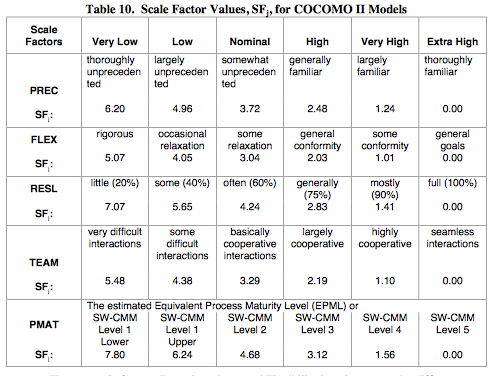
\includegraphics[trim={0.23cm 0.2cm 0.43cm 0.55cm},clip,width=\linewidth]{img/scaledriver.png}
    \caption{Scale Factor Values for COCOMO\rr II Models}
    \label{tbl:scale}
\end{figure}

\pagebreak 
In this section we will talk about COCOMO\rr II Scale Drivers. 
They are a significant source of exponential variation on a project effort. 
Each driver has a range of rating levels, from \emph{Very Low} to 
\emph{Extra High}, each with its own rate. 

\paragraph{PREC} Precedentedness. \\  % QUESTA PAROLA NON ESISTE! :/
This driver reflects the previous experience that developers have in this 
field. Actually, this is our first experience, so we think the best value for
our team is \texttt{Low}.

\paragraph{FLEX} Development flexibility. \\
This driver will change due to our flexibility degree in the development.
Our schedule is quite strict, so we choose \texttt{Low} for this project.

\paragraph{RESL} Risk resolution. \\
It reflects the extension of risk analysis. A very low value means we have done
a little analysis, high means a complete risk analysis. We choose \texttt{High}
because we did a detailed analysis (Chapter 5). 

\paragraph{TEAM} Team cohesion. \\
This value is correlated to how well the development team know each other. 
In this case we are a very cooperative team, so \texttt{Very high} value is
our choice.

\paragraph{PMAT} Process maturity. \\
This parameter reflects the process maturity of the organizazion. In particular,
this parameter has been choosen according to a weighted average of ``Yes'' answers 
to CMM Maturity Questionnaire. In our case we have chosen \texttt{High} (CMM Level 3).

\begin{table}[h!]
    \centering
\begin{tabular}{ p{5cm} | c | c }
    Scale Driver            & Factor             &  Value   \\ \hline
    Precedentedness         & \texttt{Low}       &  4.96    \\
    Development Flexibility & \texttt{Low}       &  4.05    \\
    Risk Resolution         & \texttt{High}      &  2.83    \\
    Team Cohesion           & \texttt{Very high} &  1.10    \\
    Process Maturity        & \texttt{High}      &  3.12    \\ \hline
    Total                   &                    & 16.06  
\end{tabular}
    \caption{Sum of the results}
    \label{tab:cocomo1}
\end{table}

\pagebreak
\subsection{Cost Drivers} % (fold)
These are the effort multipliers used in COCOMO\rr II model to adjust the
nominal effort. 
\label{sub:cost_drivers}

\cost{RELY}{Required Software Reliability}
{Slight inconvenience}{Easily recoverable losses}{Easily recoverable losses}
{High financial loss}{Risk to human life}{}
{0.82}{0.92}{1.00}{1.10}{1.26}{n/a} {
    This is the measure of software reliability. \texttt{Nominal} is our choice
    for this case because a downtime would not lead to high financial losses
    but will cause problems to passengers.
}
\cost{DATA}{Database Size}
{ }{D/P < 10}{$ 10 \leq D/P \le 100 $}{ $ 100 \leq D/P \le 1000 $} { $ D/P \ge 1000 $ } { }
{n/a}{0.90}{1.00}{1.14}{1.28}{n/a}
{This values tries to estimate effects that large databases could have in our application.
    We do not have a test database, so we use \emph{Nominal} as value.
}
\scost{CPLEX}{Product Complexity}
{ 0.73}{0.87}{1.00}{1.17}{1.34}{1.74} { 
    According to \cite[Table~20]{bib:cocomo2}, our software could be marked as \emph{Nominal}.
}

\cost{RUSE}{Required Reusability}
{ } { None } { Across project } { Across program } { Across product line} 
{Across multiple product lines} { n/a}{0.95}{1.00}{1.07}{1.15}{1.24} {
    Reusability is useful. Some parts should be designed as reusable (e.g.
    Mobile communication drivers). Those parts could be used not only in this project. \\
    \emph{High} is our choice here.
}

\cost{DOCU}{Documentation match to life\-cycle needs}
{Many life\-cycle needs uncovered.}{Some life\-cycle needs uncovered.}
{Right\-sized to life\-cycle needs.}{Excessive for life\-cycle needs.}
{Very excessive for life\-cycle needs.}{ } 
{0.81}{0.91}{1.00}{1.11}{1.23}{ n/a } { 
    This is a cost driver for the level of required documentation. 
    In our case it is suitable as \emph{Nominal}.
}

\pagebreak

% TODO: CONFRONTARE CON RASD SE QUESTO E' VERO
\scost{TIME}{Execution Time Constraint}
{n/a}{n/a}{1.00}{1.11}{1.29}{1.63} {
    This is a measure of the execution time constraint. We don't have strict constraints in this case, so we will set it as \emph{Low}.
}

% TODO: CONFRONTARE CON RASD SE QUESTO E' VERO
% SPAZIO INFINITO? O.o
\scost{STOR}{Main Storage Constraint}
{n/a}{n/a}{1.00}{1.05}{1.17}{1.46} {
    This is a measure of the degree of main storage constraint. 
    We don't have any constraint, so we will set it as \emph{Low}.
}

\cost{PVOL}{Platform Volatility}
{ }{Major: 12 months. Minor: 1 month.}
{ Major: 6 months. Minor: 2 weeks } { Major: 2 months. Minor: 1 weeks }
{ Major: 2 weeks. Minor: 2 days } { }
{n/a}{0.87}{1.00}{1.15}{1.30}{n/a} {
    Our estimation is that this is a stable system with low volatility.
    \emph{Low} is a good choice here.
}

\scost{ACAP}{Analyst Capability}
{1.42}{1.19}{1.00}{0.85}{0.71}{n/a} {
    This driver should be set to \emph{High} since we dedicated a lot of
    effort in analysing the problem requirements.
}

\scost{PCAP}{Programmer Capability}
{1.34}{1.15}{1.00}{0.88}{0.76}{n/a} {
    This driver should emphasize our programmers' capabilites as a team. 
    Our cooperation is quite good, so we set it as \emph{High}.
}

\cost{APEX}{Application Experience}
{ $ \leq $ 2 months } { 6 months } {1 year } {3 years} {6 years} { }
{1.22}{1.10}{1.00}{0.88}{0.81}{n/a} { 
    Our experience in this field is very low. So we think that a good estimate
    will happen if we set this value to \emph {Very Low}.
}

\cost{PLEX}{Platform Experience}
{ $ \leq $ 2 months } { 6 months } {1 year } {3 years} {6 years} { }
{1.19}{1.09}{1.00}{0.91}{0.85}{n/a} { 
    Our average knowledge about platforms as databases, UI, client/server architecture
    is around 1 year. We set this value as \emph{Nominal}.
}

\cost{LTEX}{Language and Tool Experience}
{ $ \leq $ 2 months } { 6 months } {1 year } {3 years} {6 years} { }
{1.20}{1.09}{1.00}{0.91}{0.84}{n/a} { 
    This is like the previous parameter. Our experience is around one year,
    so this value will be set to \emph{Nominal}.
}
\pagebreak
\cost{PCON}{Personnel continuity}
{48 \% / year} { 24 \% / year} { 12 \% / year} { 6 \% / year} { 3 \% / year} { }
{1.29}{1.12}{1.00}{0.90}{0.81}{n/a} { 
    We can estimate a \emph{High} personnel continuity.
}

\cost{TOOL}{Use of software tools}
{Edit, code, debug}
{Simple, frontend, backend CASE, little integration}
{Basic lifecycle tools, moderately integrated}
{Strong, mature lifecycle tools, moderately integrated}
{Strong, mature, proactive lifecycle tools, well integrated with processes, methods, reuse}
{ }
{1.17}{1.09}{1.00}{0.90}{0.78}{n/a} { 
    We are going to use basic tools like Eclipse as IDE, Maven as dependency manager
    and GIT as versioning tool. So we think that \emph{Nominal} will be good for us.
}

\pagebreak
\cost{SITE}{Multisite development}
{Some phone, mail}
{Individual phone, FAX}
{Narrowband email}
{Wideband electronic communication}
{Wideband elect. comm, occasional video conf.}
{Interactive multimedia}
{1.22}{1.09}{1.00}{0.93}{0.86}{0.80} { 
    We are going to use chats, emails and phone calls.
    So we choose \emph{High} here.
}

\cost{SCED}{Required development schedule}
{75\% of nominal}
{85\% of nominal}
{100\% of nominal}
{130\% of nominal}
{160\% of nominal}
{}
{1.43}{1.14}{1.00}{1.00}{1.00}{n/a} { 
    One hundred percent is good for us. So we will choose \emph{Nominal} here.
}

\pagebreak

\paragraph{Product} 
Now we can compute the product of all Cost Drivers.

\begin{table}[h!]
    \centering
\begin{tabular}{| p{8cm} | c | c |} \hline
Cost Driver                               & Factor             &  Value   \\ \hline 
Required Software Reliability             & \texttt{Nominal}   &  1.00    \\
Database Size                             & \texttt{Nominal}   &  1.00    \\
Product Complexity                        & \texttt{Nominal}   &  1.00    \\
Required Reusability                      & \texttt{High}      &  1.07    \\
Documentation match to life\-cycle needs  & \texttt{Nominal}   &  1.00    \\
Execution Time Constraint                 & \texttt{Low}       &   n/a    \\
Main Storage Constraint                   & \texttt{Low}       &   n/a    \\
Platform Volatility                       & \texttt{Low}       &  0.87    \\
Analyst Capability                        & \texttt{High}      &  0.85    \\  
Programmer Capability                     & \texttt{High}      &  0.88    \\  
Application Experience                    & \texttt{Very Low}  &  1.22    \\  
Platform Experience                       & \texttt{Nominal}   &  1.00    \\  
Language and Tool Experience              & \texttt{Nominal}   &  1.00    \\  
Personnel continuity                      & \texttt{High}      &  0.90    \\  
Use of software tools                     & \texttt{Nominal}   &  1.00    \\  
Multisite development                     & \texttt{High}      &  0.93    \\   
Required development schedule             & \texttt{Nominal}   &  1.00    \\ \hline
Product                                   &                    &  0.71    \\ \hline
\end{tabular}
\caption{Product between Cost driver results}
\label{tab:cocomo2}
\end{table}

\pagebreak
\subsection{Effort Equation} % (fold)
\label{sub:effort_equation}

Now, having both cost drivers product and scale drivers factors we can compute
the effort, in Person-Month with the following equation:
$$ Effort = A * EAF * KSLOC^E $$

Where $A$ is the COCOMO\rr 2000 constant, $ A = 2.94 $. $EAF$ is the product of
all cost drivers. In our case it is $ EAF = 0.71 $. Using function points estimation
we can say that $ KSLOC = 8.694 $.
Last thing: $E$ is the exponent derived from Scale Drivers. It is calculated with
the following formula:

$$ E = B + 0.01 * \sum_{i=1}^5 SF_i $$

Where $ B = 0.91 $ in COCOMO\rr 2000.
In our project, we can derive that $ E = 0.91 + 0.01 * 16.06 = 0.91 + 0.1606 \cong 1.07 $.

Using this parameter, we can compute our effort:

$$ Effort = 2.94 * 0.71 * 8.694^{1.07} = 21.11~PM $$

\subsection{Schedule Estimation}
\label{sub:schedule_estimation}

Now we can estimate the project duration with the following equation:
$$ Duration = 3.67 * Effort^F $$

Where $Effort$ is the estimated effort and $SE$ is the schedule equation exponent derived
from the five Scale Drivers.
We can obtain $SE$ using the following formula:
$$ F = D + 0.2 * 0.01 * \sum_{i=1}^5 SF_i = 0.28 + 0.2 * 0.01 * 16.06 \cong 0.31 $$
$$ Duration = 3.67 * 21.11^F = 3.67 * 21.11^{0.31} \cong 9.44~Months $$

